\documentclass[a4paper,12pt]{extarticle}
\usepackage[utf8x]{inputenc}
\usepackage[T1,T2A]{fontenc}
\usepackage[russian]{babel}
\usepackage{hyperref}
\usepackage{indentfirst}
\usepackage{listings}
\usepackage{color}
\usepackage{here}
\usepackage{array}
\usepackage{multirow}
\usepackage{graphicx}
\usepackage{amsmath}
%\usepackage[dvips]{graphicx}

\usepackage{caption}
\renewcommand{\lstlistingname}{Программа} % заголовок листингов кода

\bibliographystyle{ugost2008ls}

\lstset{ %
extendedchars=\true,
keepspaces=true,
language=C,						% choose the language of the code
basicstyle=\footnotesize,		% the size of the fonts that are used for the code
numbers=left,					% where to put the line-numbers
numberstyle=\footnotesize,		% the size of the fonts that are used for the line-numbers
stepnumber=1,					% the step between two line-numbers. If it is 1 each line will be numbered
numbersep=5pt,					% how far the line-numbers are from the code
backgroundcolor=\color{white},	% choose the background color. You must add \usepackage{color}
showspaces=false				% show spaces adding particular underscores
showstringspaces=false,			% underline spaces within strings
showtabs=false,					% show tabs within strings adding particular underscores
frame=single,           		% adds a frame around the code
tabsize=2,						% sets default tabsize to 2 spaces
captionpos=t,					% sets the caption-position to top
breaklines=true,				% sets automatic line breaking
breakatwhitespace=false,		% sets if automatic breaks should only happen at whitespace
escapeinside={\%*}{*)},			% if you want to add a comment within your code
postbreak=\raisebox{0ex}[0ex][0ex]{\ensuremath{\color{red}\hookrightarrow\space}},
texcl=true,
%inputpath=listings,                     % директория с листингами
}

\usepackage[left=2cm,right=2cm,
top=2cm,bottom=2cm,bindingoffset=0cm]{geometry}

%% Нумерация картинок по секциям
\usepackage{chngcntr}
\counterwithin{figure}{section}
\counterwithin{table}{section}

%%Точки нумерации заголовков
\usepackage{titlesec}
\titlelabel{\thetitle.\quad}
\usepackage[dotinlabels]{titletoc}

%% Оформления подписи рисунка
\addto\captionsrussian{\renewcommand{\figurename}{Рисунок}}
\captionsetup[figure]{labelsep = period}

%% Подпись таблицы
\DeclareCaptionFormat{hfillstart}{\hfill#1#2#3\par}
\captionsetup[table]{format=hfillstart,labelsep=newline,justification=centering,skip=-10pt,textfont=bf}

%% Путь к каталогу с рисунками
%\graphicspath{{fig/}}

%% Внесение titlepage в учёт счётчика страниц
\makeatletter
\renewenvironment{titlepage} {
 \thispagestyle{empty}
}
\makeatother

\begin{document}	% начало документа

% Титульная страница
\begin{titlepage}	% начало титульной страницы

	\begin{center}		% выравнивание по центру

		\large Санкт-Петербургский политехнический университет Петра Великого\\
		\large Институт компьютерных наук и технологий \\
		\large Высшая школа интеллектуальных систем и суперкомпьютерных технологий\\[6cm]
		% название института, затем отступ 6см

		\huge Алгоритмы цифровой обработки изображений\\[0.5cm] % название работы, затем отступ 0,5см
		\large Отчет по лабораторной работе №3 \\[0.1cm]
		\large Алгоритмы сглаживания изображений \\[5cm]

	\end{center}


	\begin{flushright} % выравнивание по правому краю
		\begin{minipage}{0.25\textwidth} % врезка в половину ширины текста
			\begin{flushleft} % выровнять её содержимое по левому краю

				\large\textbf{Работу выполнил:}\\
				\large Медведев А.В.\\
				\large {Группа:} 3540901/01502\\

				\large \textbf{Преподаватель:}\\
				\large Абрамов Н.А.

			\end{flushleft}
		\end{minipage}
	\end{flushright}

	\vfill % заполнить всё доступное ниже пространство

	\begin{center}
	\large Санкт-Петербург\\
	\large \the\year % вывести дату
	\end{center} % закончить выравнивание по центру

\end{titlepage} % конец титульной страницы

\vfill % заполнить всё доступное ниже пространство

% Содержание
% Содержание
\renewcommand\contentsname{\centerline{Содержание}}
\tableofcontents
\newpage


\section{Цель работы}

Ознакомление с морфологическими операциями.

\section{Программа работы}
\subsection{Бинаризация изображения}
\subsection{Наращивание / дилетация}
\subsection{Эрозия}
\subsection{Морфологическое открытие / размыкание}
\subsection{Морфологическое закрытие / замыкание}

\section{Ход выполнения работы}

\subsection{Бинаризация изображения}

Бинаризация изображения — преобразование исходного изображе-ния в градациях серого в бинарное изображение, элементы которогомогут принимать только два значения.

Ниже представлено исходное изображение и его бинаризированный вариант, который будет использоваться далее в лабораторной работе.

\begin{figure}[H]
	\begin{minipage}[h]{0.49\linewidth}
		\center{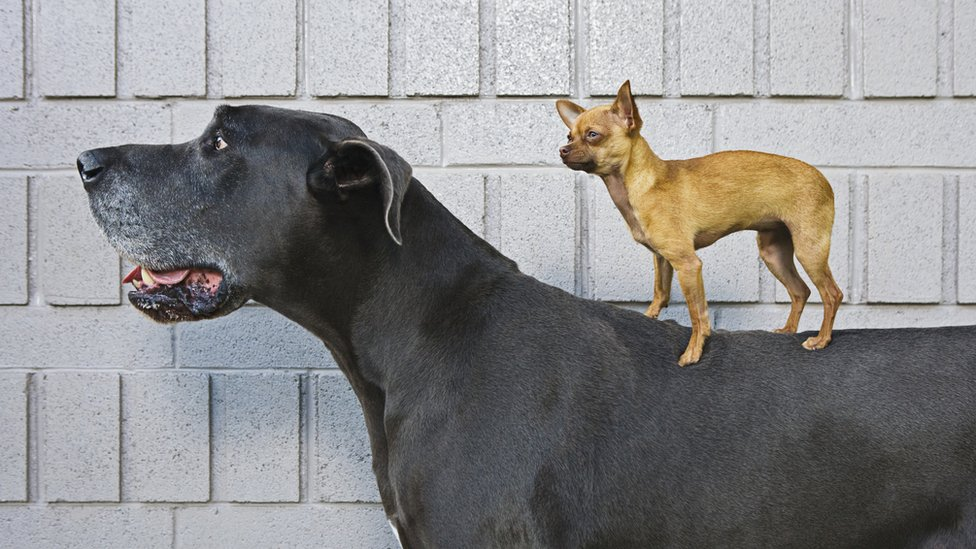
\includegraphics[width=1\linewidth]{../resources/1/source} \\ Исходное изображени}
	\end{minipage}
	\hfill
	\begin{minipage}[h]{0.49\linewidth}
		\center{\includegraphics[width=1\linewidth]{../out/1/3/binarized_img} \\ Бинаризованное изображение}
	\end{minipage}
\end{figure}

\newpage

\subsection{Наращивание / дилетация}

Данная операция производится следующим образом: 

Структурный элемент применяется ко всем пикселам бинарного изображения. Каждый раз, когда центр структурного элемента совмещается с единичным бинарным пикселом, ко всем соответствующим пикселам бинарного изображения применяется логическое сложение с пикселами структурного элемента.  Результаты логического сложения записываются в выходное бинарное изображение.

Ниже представлены результаты применения данного метода с различными параметрами размера структурного элемента к исходному бинаризированному изображению.

\begin{figure}[H]
	\begin{minipage}[h]{0.49\linewidth}
		\center{\includegraphics[width=1\linewidth]{../out/1/3/binarized_img} \\ Исходное изображени}
	\end{minipage}
	\hfill
	\begin{minipage}[h]{0.49\linewidth}
		\center{\includegraphics[width=1\linewidth]{../out/1/3/escalating_img} \\ 3х3}
	\end{minipage}
	\vfill
	\begin{minipage}[h]{0.49\linewidth}
		\center{\includegraphics[width=1\linewidth]{../out/1/5/escalating_img} \\ 5х5}
	\end{minipage}
	\hfill
	\begin{minipage}[h]{0.49\linewidth}
		\center{\includegraphics[width=1\linewidth]{../out/1/7/escalating_img} \\ 7х7}
	\end{minipage}
\end{figure}

\newpage

\subsection{Эрозия}

Данная операция производится следующим образом: 

Структурный элемент проходит по всем пикселам бинаризированного изображения. Если в некоторой позиции каждый пиксел структурного элемента совпадает с единичным пикселом бинарного изображения, то выполняется логическое сложение центрального пиксела структурного элемента с соответствующим пикселом выходного изображения. 

В результате применения эрозии все объекты, меньшие чем структурный элемент, стираются, объекты, соединённые тонкими линиями становятся разъединёнными и размеры всех объектов уменьшаются.

Ниже представлены результаты применения данного метода с различными параметрами размера структурного элемента к исходному бинаризированному изображению.

\begin{figure}[H]
	\begin{minipage}[h]{0.49\linewidth}
		\center{\includegraphics[width=1\linewidth]{../out/1/3/binarized_img} \\ Исходное изображени}
	\end{minipage}
	\hfill
	\begin{minipage}[h]{0.49\linewidth}
		\center{\includegraphics[width=1\linewidth]{../out/1/3/erosion_img} \\ Структурный элемент размера 3х3}
	\end{minipage}
	\vfill
	\begin{minipage}[h]{0.49\linewidth}
		\center{\includegraphics[width=1\linewidth]{../out/1/5/erosion_img} \\ Структурный элемент размера 5х5}
	\end{minipage}
	\hfill
	\begin{minipage}[h]{0.49\linewidth}
		\center{\includegraphics[width=1\linewidth]{../out/1/7/erosion_img} \\ Структурный элемент размера 7х7}
	\end{minipage}
\end{figure}

\newpage

\subsection{Морфологическое открытие / размыкание}

Операция эрозии полезна для удаления малых объектов и различных шумов, но у этой операции есть недостаток – все остающиеся объекты уменьшаются в размере. Этого эффекта можно избежать, если после операции эрозии применить операцию наращивания с тем же структурным элементом.

Размыкание отсеивает все объекты, меньшие чем структурный элемент, но при этом помогает избежать сильного уменьшения размера объектов. Также размыкание идеально подходит для удаления линий, толщина которых меньше, чем диаметр структурного элемента. Также важно помнить, что после этой операции контуры объектов становятся более гладкими.

Ниже представлены результаты применения данного метода с различными параметрами размера структурного элемента к исходному бинаризированному изображению.

\begin{figure}[H]
	\begin{minipage}[h]{0.49\linewidth}
		\center{\includegraphics[width=1\linewidth]{../out/1/3/binarized_img} \\ Исходное изображени}
	\end{minipage}
	\hfill
	\begin{minipage}[h]{0.49\linewidth}
		\center{\includegraphics[width=1\linewidth]{../out/1/3/morphological_discovery_img} \\ Структурный элемент размера 3х3}
	\end{minipage}
	\vfill
	\begin{minipage}[h]{0.49\linewidth}
		\center{\includegraphics[width=1\linewidth]{../out/1/5/morphological_discovery_img} \\ Структурный элемент размера 5х5}
	\end{minipage}
	\hfill
	\begin{minipage}[h]{0.49\linewidth}
		\center{\includegraphics[width=1\linewidth]{../out/1/7/morphological_discovery_img} \\ Структурный элемент размера 7х7}
	\end{minipage}
\end{figure}

\newpage

\subsection{Морфологическое закрытие / замыкание}

Если к изображению применить сначала операцию наращивания, то мы сможем избавиться от малых дыр и щелей, но при этом произойдёт увеличение контура объекта. Избежать этого увеличения позволяет операция эрозия, выполненная сразу после наращивания с тем же структурным элементом.

Ниже представлены результаты применения данного метода с различными параметрами размера структурного элемента к исходному бинаризированному изображению.

\begin{figure}[H]
	\begin{minipage}[h]{0.49\linewidth}
		\center{\includegraphics[width=1\linewidth]{../out/1/3/binarized_img} \\ Исходное изображени}
	\end{minipage}
	\hfill
	\begin{minipage}[h]{0.49\linewidth}
		\center{\includegraphics[width=1\linewidth]{../out/1/3/morphological_closure_img} \\ Структурный элемент размера 3х3}
	\end{minipage}
	\vfill
	\begin{minipage}[h]{0.49\linewidth}
		\center{\includegraphics[width=1\linewidth]{../out/1/5/morphological_closure_img} \\ Структурный элемент размера 5х5}
	\end{minipage}
	\hfill
	\begin{minipage}[h]{0.49\linewidth}
		\center{\includegraphics[width=1\linewidth]{../out/1/7/morphological_closure_img} \\ Структурный элемент размера 7х7}
	\end{minipage}
\end{figure}


\section{Вывод}

В данной лабораторной работе были рассмотрены следующие орфологические операции: дилетация, эрозия, морфологическое открытие, морфологическое закрытие. Они помогают удалить с изображения мелкие объекты и разлицные шумы, дыры и щели. Совместное выполнение дилетации и эрозии на одном изображении помогает устранить недостатки, которые имеют данные операции при выполнении по отдельности.

\vfill % заполнить всё доступное ниже пространство

\newpage
\section{Листинг}

\lstinputlisting[
label=code:equalization,
]{../main.py}
\parindent=1cm

\end{document}
